% ----------------------------------------------------------------------
%
%                            TFMTesis.tex
%
%----------------------------------------------------------------------
%
% Este fichero contiene el "documento maestro" del documento. Lo único
% que hace es configurar el entorno LaTeX e incluir los ficheros .tex
% que contienen cada sección.
%
%----------------------------------------------------------------------
%
% Los ficheros necesarios para este documento son:
%
%       TeXiS/* : ficheros de la plantilla TeXiS.
%       Cascaras/* : ficheros con las partes del documento que no
%          son capítulos ni apéndices (portada, agradecimientos, etc.)
%       Capitulos/*.tex : capítulos de la tesis
%       Apendices/*.tex: apéndices de la tesis
%       constantes.tex: constantes LaTeX
%       config.tex : configuración de la "compilación" del documento
%       guionado.tex : palabras con guiones
%
% Para la bibliografía, además, se necesitan:
%
%       *.bib : ficheros con la información de las referencias
%
% ---------------------------------------------------------------------

\documentclass[12pt,a4paper,twoside]{book}

%
% Definimos  el   comando  \compilaCapitulo,  que   luego  se  utiliza
% (opcionalmente) en config.tex. Quedaría  mejor si también se definiera
% en  ese fichero,  pero por  el modo  en el  que funciona  eso  no es
% posible. Puedes consultar la documentación de ese fichero para tener
% más  información. Definimos también  \compilaApendice, que  tiene el
% mismo  cometido, pero  que se  utiliza para  compilar  únicamente un
% apéndice.
%
%
% Si  queremos   compilar  solo   una  parte  del   documento  podemos
% especificar mediante  \includeonly{...} qué ficheros  son los únicos
% que queremos  que se incluyan.  Esto  es útil por  ejemplo para sólo
% compilar un capítulo.
%
% El problema es que todos aquellos  ficheros que NO estén en la lista
% NO   se  incluirán...  y   eso  también   afecta  a   ficheros  de
% la plantilla...
%
% Total,  que definimos  una constante  con los  ficheros  que siempre
% vamos a querer compilar  (aquellos relacionados con configuración) y
% luego definimos \compilaCapitulo.
\newcommand{\ficherosBasicosTeXiS}{%
TeXiS/TeXiS_pream,TeXiS/TeXiS_cab,TeXiS/TeXiS_bib,TeXiS/TeXiS_cover%
}
\newcommand{\ficherosBasicosTexto}{%
constantes,guionado,Cascaras/bibliografia,config%
}
\newcommand{\compilaCapitulo}[1]{%
\includeonly{\ficherosBasicosTeXiS,\ficherosBasicosTexto,Capitulos/#1}%
}

\newcommand{\compilaApendice}[1]{%
\includeonly{\ficherosBasicosTeXiS,\ficherosBasicosTexto,Apendices/#1}%
}

%- - - - - - - - - - - - - - - - - - - - - - - - - - - - - - - - - - -
%            Preámbulo del documento. Configuraciones varias
%- - - - - - - - - - - - - - - - - - - - - - - - - - - - - - - - - - -

% Define  el  tipo  de  compilación que  estamos  haciendo.   Contiene
% definiciones  de  constantes que  cambian  el  comportamiento de  la
% compilación. Debe incluirse antes del paquete TeXiS/TeXiS.sty
%---------------------------------------------------------------------
%
%                          config.tex
%
%---------------------------------------------------------------------
%
% Contiene la  definición de constantes  que determinan el modo  en el
% que se compilará el documento.
%
%---------------------------------------------------------------------
%
% En concreto, podemos  indicar si queremos "modo release",  en el que
% no  aparecerán  los  comentarios  (creados  mediante  \com{Texto}  o
% \comp{Texto}) ni los "por  hacer" (creados mediante \todo{Texto}), y
% sí aparecerán los índices. El modo "debug" (o mejor dicho en modo no
% "release" muestra los índices  (construirlos lleva tiempo y son poco
% útiles  salvo  para   la  versión  final),  pero  sí   el  resto  de
% anotaciones.
%
% Si se compila con LaTeX (no  con pdflatex) en modo Debug, también se
% muestran en una esquina de cada página las entradas (en el índice de
% palabras) que referencian  a dicha página (consulta TeXiS_pream.tex,
% en la parte referente a show).
%
% El soporte para  el índice de palabras en  TeXiS es embrionario, por
% lo  que no  asumas que  esto funcionará  correctamente.  Consulta la
% documentación al respecto en TeXiS_pream.tex.
%
%
% También  aquí configuramos  si queremos  o  no que  se incluyan  los
% acrónimos  en el  documento final  en la  versión release.  Para eso
% define (o no) la constante \acronimosEnRelease.
%
% Utilizando \compilaCapitulo{nombre}  podemos también especificar qué
% capítulo(s) queremos que se compilen. Si no se pone nada, se compila
% el documento  completo.  Si se pone, por  ejemplo, 01Introduccion se
% compilará únicamente el fichero Capitulos/01Introduccion.tex
%
% Para compilar varios  capítulos, se separan sus nombres  con comas y
% no se ponen espacios de separación.
%
% En realidad  la macro \compilaCapitulo  está definida en  el fichero
% principal tesis.tex.
%
%---------------------------------------------------------------------


% Comentar la línea si no se compila en modo release.
% TeXiS hará el resto.
% ¡¡¡Si cambias esto, haz un make clean antes de recompilar!!!
\def\release{1}


% Descomentar la linea si se quieren incluir los
% acrónimos en modo release (en modo debug
% no se incluirán nunca).
% ¡¡¡Si cambias esto, haz un make clean antes de recompilar!!!
%\def\acronimosEnRelease{1}


% Descomentar la línea para establecer el capítulo que queremos
% compilar

% \compilaCapitulo{01Introduccion}
% \compilaCapitulo{02EstructuraYGeneracion}
% \compilaCapitulo{03Edicion}
% \compilaCapitulo{04Imagenes}
% \compilaCapitulo{05Bibliografia}
% \compilaCapitulo{06Makefile}

% \compilaApendice{01AsiSeHizo}

% Variable local para emacs, para  que encuentre el fichero maestro de
% compilación y funcionen mejor algunas teclas rápidas de AucTeX
%%%
%%% Local Variables:
%%% mode: latex
%%% TeX-master: "./Tesis.tex"
%%% End:


% Paquete de la plantilla
\usepackage{TeXiS/TeXiS}

% Incluimos el fichero con comandos de constantes
%---------------------------------------------------------------------
%
%                          constantes.tex
%
%---------------------------------------------------------------------
%
% Fichero que  declara nuevos comandos LaTeX  sencillos realizados por
% comodidad en la escritura de determinadas palabras
%
%---------------------------------------------------------------------

%%%%%%%%%%%%%%%%%%%%%%%%%%%%%%%%%%%%%%%%%%%%%%%%%%%%%%%%%%%%%%%%%%%%%%
% Comando: 
%
%       \titulo
%
% Resultado: 
%
% Escribe el título del documento.
%%%%%%%%%%%%%%%%%%%%%%%%%%%%%%%%%%%%%%%%%%%%%%%%%%%%%%%%%%%%%%%%%%%%%%
\def\titulo{\textsc{TeXiS}: Desarrollo de una herramienta basada en lenguaje de apoyo a la terapia basada en reminiscencia}

%%%%%%%%%%%%%%%%%%%%%%%%%%%%%%%%%%%%%%%%%%%%%%%%%%%%%%%%%%%%%%%%%%%%%%
% Comando: 
%
%       \autor
%
% Resultado: 
%
% Escribe el autor del documento.
%%%%%%%%%%%%%%%%%%%%%%%%%%%%%%%%%%%%%%%%%%%%%%%%%%%%%%%%%%%%%%%%%%%%%%
\def\autor{Marta Vicente Navarro}

% Variable local para emacs, para  que encuentre el fichero maestro de
% compilación y funcionen mejor algunas teclas rápidas de AucTeX

%%%
%%% Local Variables:
%%% mode: latex
%%% TeX-master: "tesis.tex"
%%% End:


% Sacamos en el log de la compilación el copyright
%\typeout{Copyright Marco Antonio and Pedro Pablo Gomez Martin}

%
% "Metadatos" para el PDF
%
\usepackage{xcolor}
% Definición del estilo Spyder
\definecolor{spyder_keyword}{RGB}{140, 0, 255} % Color de las palabras clave
\definecolor{spyder_comment}{RGB}{63, 127, 95} % Color de los comentarios
\definecolor{spyder_string}{RGB}{206, 145, 120} % Color de las cadenas
\definecolor{spyder_background}{RGB}{255, 255, 255} % Color de fondo del código
\definecolor{spyder_frame}{RGB}{200, 200, 200} % Color del marco del código

\lstdefinestyle{SpyderStyle}{
	language=Python,
	basicstyle=\ttfamily,
	keywordstyle=\color{spyder_keyword},
	commentstyle=\color{spyder_comment},
	stringstyle=\color{spyder_string},
	backgroundcolor=\color{spyder_background},
	frame=single,
	framerule=0.5pt,
	framesep=3pt,
}
\ifpdf\hypersetup{%
    pdftitle = {\titulo},
    pdfsubject = {Plantilla de Tesis},
    pdfkeywords = {Plantilla, LaTeX, tesis, trabajo de
      investigación, trabajo de Master},
    pdfauthor = {\textcopyright\ \autor},
    pdfcreator = {\LaTeX\ con el paquete \flqq hyperref\frqq},
    pdfproducer = {pdfeTeX-0.\the\pdftexversion\pdftexrevision},
    }
    
\fi

%- - - - - - - - - - - - - - - - - - - - - - - - - - - - - - - - - - -
%                        Documento
%- - - - - - - - - - - - - - - - - - - - - - - - - - - - - - - - - - -
\begin{document}

% Incluimos el  fichero de definición de guionado  de algunas palabras
% que LaTeX no ha dividido como debería
%----------------------------------------------------------------
%
%                          guionado.tex
%
%----------------------------------------------------------------
%
% Fichero con algunas divisiones de palabras que LaTeX no
% hace correctamente si no se le da alguna ayuda.
%
%----------------------------------------------------------------

\hyphenation{
% a
abs-trac-to
abs-trac-tos
abs-trac-ta
abs-trac-tas
ac-tua-do-res
a-gra-de-ci-mien-tos
ana-li-za-dor
an-te-rio-res
an-te-rior-men-te
apa-rien-cia
a-pro-pia-do
a-pro-pia-dos
a-pro-pia-da
a-pro-pia-das
a-pro-ve-cha-mien-to
a-que-llo
a-que-llos
a-que-lla
a-que-llas
a-sig-na-tu-ra
a-sig-na-tu-ras
a-so-cia-da
a-so-cia-das
a-so-cia-do
a-so-cia-dos
au-to-ma-ti-za-do
% b
batch
bi-blio-gra-fía
bi-blio-grá-fi-cas
bien
bo-rra-dor
boo-l-ean-expr
% c
ca-be-ce-ra
call-me-thod-ins-truc-tion
cas-te-lla-no
cir-cuns-tan-cia
cir-cuns-tan-cias
co-he-ren-te
co-he-ren-tes
co-he-ren-cia
co-li-bri
co-men-ta-rio
co-mer-cia-les
co-no-ci-mien-to
cons-cien-te
con-si-de-ra-ba
con-si-de-ra-mos
con-si-de-rar-se
cons-tan-te
cons-trucción
cons-tru-ye
cons-tru-ir-se
con-tro-le
co-rrec-ta-men-te
co-rres-pon-den
co-rres-pon-dien-te
co-rres-pon-dien-tes
co-ti-dia-na
co-ti-dia-no
crean
cris-ta-li-zan
cu-rri-cu-la
cu-rri-cu-lum
cu-rri-cu-lar
cu-rri-cu-la-res
% d
de-di-ca-do
de-di-ca-dos
de-di-ca-da
de-di-ca-das
de-rro-te-ro
de-rro-te-ros
de-sa-rro-llo
de-sa-rro-llos
de-sa-rro-lla-do
de-sa-rro-lla-dos
de-sa-rro-lla-da
de-sa-rro-lla-das
de-sa-rro-lla-dor
de-sa-rro-llar
des-cri-bi-re-mos
des-crip-ción
des-crip-cio-nes
des-cri-to
des-pués
de-ta-lla-do
de-ta-lla-dos
de-ta-lla-da
de-ta-lla-das
di-a-gra-ma
di-a-gra-mas
di-se-ños
dis-po-ner
dis-po-ni-bi-li-dad
do-cu-men-ta-da
do-cu-men-to
do-cu-men-tos
% e
edi-ta-do
e-du-ca-ti-vo
e-du-ca-ti-vos
e-du-ca-ti-va
e-du-ca-ti-vas
e-la-bo-ra-do
e-la-bo-ra-dos
e-la-bo-ra-da
e-la-bo-ra-das
es-co-llo
es-co-llos
es-tu-dia-do
es-tu-dia-dos
es-tu-dia-da
es-tu-dia-das
es-tu-dian-te
e-va-lua-cio-nes
e-va-lua-do-res
exis-ten-tes
exhaus-ti-va
ex-pe-rien-cia
ex-pe-rien-cias
% f
for-ma-li-za-do
% g
ge-ne-ra-ción
ge-ne-ra-dor
ge-ne-ra-do-res
ge-ne-ran
% h
he-rra-mien-ta
he-rra-mien-tas
% i
i-dio-ma
i-dio-mas
im-pres-cin-di-ble
im-pres-cin-di-bles
in-de-xa-do
in-de-xa-dos
in-de-xa-da
in-de-xa-das
in-di-vi-dual
in-fe-ren-cia
in-fe-ren-cias
in-for-ma-ti-ca
in-gre-dien-te
in-gre-dien-tes
in-me-dia-ta-men-te
ins-ta-la-do
ins-tan-cias
% j
% k
% l
len-gua-je
li-be-ra-to-rio
li-be-ra-to-rios
li-be-ra-to-ria
li-be-ra-to-rias
li-mi-ta-do
li-te-ra-rio
li-te-ra-rios
li-te-ra-ria
li-te-ra-rias
lo-tes
% m
ma-ne-ra
ma-nual
mas-que-ra-de
ma-yor
me-mo-ria
mi-nis-te-rio
mi-nis-te-rios
mo-de-lo
mo-de-los
mo-de-la-do
mo-du-la-ri-dad
mo-vi-mien-to
% n
na-tu-ral
ni-vel
nues-tro
% o
obs-tan-te
o-rien-ta-do
o-rien-ta-dos
o-rien-ta-da
o-rien-ta-das
% p
pa-ra-le-lo
pa-ra-le-la
par-ti-cu-lar
par-ti-cu-lar-men-te
pe-da-gó-gi-ca
pe-da-gó-gi-cas
pe-da-gó-gi-co
pe-da-gó-gi-cos
pe-rio-di-ci-dad
per-so-na-je
plan-te-a-mien-to
plan-te-a-mien-tos
po-si-ción
pre-fe-ren-cia
pre-fe-ren-cias
pres-cin-di-ble
pres-cin-di-bles
pri-me-ra
pro-ble-ma
pro-ble-mas
pró-xi-mo
pu-bli-ca-cio-nes
pu-bli-ca-do
% q
% r
rá-pi-da
rá-pi-do
ra-zo-na-mien-to
ra-zo-na-mien-tos
re-a-li-zan-do
re-fe-ren-cia
re-fe-ren-cias
re-fe-ren-cia-da
re-fe-ren-cian
re-le-van-tes
re-pre-sen-ta-do
re-pre-sen-ta-dos
re-pre-sen-ta-da
re-pre-sen-ta-das
re-pre-sen-tar-lo
re-qui-si-to
re-qui-si-tos
res-pon-der
res-pon-sa-ble
% s
se-pa-ra-do
si-guien-do
si-guien-te
si-guien-tes
si-guie-ron
si-mi-lar
si-mi-la-res
si-tua-ción
% t
tem-pe-ra-ments
te-ner
trans-fe-ren-cia
trans-fe-ren-cias
% u
u-sua-rio
Unreal-Ed
% v
va-lor
va-lo-res
va-rian-te
ver-da-de-ro
ver-da-de-ros
ver-da-de-ra
ver-da-de-ras
ver-da-de-ra-men-te
ve-ri-fi-ca
% w
% x
% y
% z
}
% Variable local para emacs, para que encuentre el fichero
% maestro de compilación
%%%
%%% Local Variables:
%%% mode: latex
%%% TeX-master: "./Tesis.tex"
%%% End:


% Marcamos  el inicio  del  documento para  la  numeración de  páginas
% (usando números romanos para esta primera fase).
\frontmatter
\pagestyle{empty}

%---------------------------------------------------------------------
%
%                          configCover.tex
%
%---------------------------------------------------------------------
%
% cover.tex
% Copyright 2009 Marco Antonio Gomez-Martin, Pedro Pablo Gomez-Martin
%
% This file belongs to the TeXiS manual, a LaTeX template for writting
% Thesis and other documents. The complete last TeXiS package can
% be obtained from http://gaia.fdi.ucm.es/projects/texis/
%
% Although the TeXiS template itself is distributed under the 
% conditions of the LaTeX Project Public License
% (http://www.latex-project.org/lppl.txt), the manual content
% uses the CC-BY-SA license that stays that you are free:
%
%    - to share & to copy, distribute and transmit the work
%    - to remix and to adapt the work
%
% under the following conditions:
%
%    - Attribution: you must attribute the work in the manner
%      specified by the author or licensor (but not in any way that
%      suggests that they endorse you or your use of the work).
%    - Share Alike: if you alter, transform, or build upon this
%      work, you may distribute the resulting work only under the
%      same, similar or a compatible license.
%
% The complete license is available in
% http://creativecommons.org/licenses/by-sa/3.0/legalcode
%
%---------------------------------------------------------------------
%
% Fichero que contiene la configuración de la portada y de la 
% primera hoja del documento.
%
%---------------------------------------------------------------------


% Pueden configurarse todos los elementos del contenido de la portada
% utilizando comandos.

%%%%%%%%%%%%%%%%%%%%%%%%%%%%%%%%%%%%%%%%%%%%%%%%%%%%%%%%%%%%%%%%%%%%%%
% Título del documento:
% \tituloPortada{titulo}
% Nota:
% Si no se define se utiliza el del \titulo. Este comando permite
% cambiar el título de forma que se especifiquen dónde se quieren
% los retornos de carro cuando se utilizan fuentes grandes.
%%%%%%%%%%%%%%%%%%%%%%%%%%%%%%%%%%%%%%%%%%%%%%%%%%%%%%%%%%%%%%%%%%%%%%
\tituloPortada{Desarrollo de un chatbot de apoyo a la terapia basada en reminiscencia }


%%%%%%%%%%%%%%%%%%%%%%%%%%%%%%%%%%%%%%%%%%%%%%%%%%%%%%%%%%%%%%%%%%%%%%
% Título del documento en inglés:
% \tituloPortadaEng{titulo}
% Nota:
% Si no se define se utiliza el del \titulo. Este comando permite
% cambiar el título de forma que se especifiquen dónde se quieren
% los retornos de carro cuando se utilizan fuentes grandes.
%%%%%%%%%%%%%%%%%%%%%%%%%%%%%%%%%%%%%%%%%%%%%%%%%%%%%%%%%%%%%%%%%%%%%%
\tituloPortadaEng{A chatbot to support reminiscence therapy}

%%%%%%%%%%%%%%%%%%%%%%%%%%%%%%%%%%%%%%%%%%%%%%%%%%%%%%%%%%%%%%%%%%%%%%
% Autor del documento:
% \autorPortada{Nombre}
% Se utiliza en la portada y en el valor por defecto del
% primer subtítulo de la segunda portada.
%%%%%%%%%%%%%%%%%%%%%%%%%%%%%%%%%%%%%%%%%%%%%%%%%%%%%%%%%%%%%%%%%%%%%%
\autorPortada{Marta Vicente Navarro}

%%%%%%%%%%%%%%%%%%%%%%%%%%%%%%%%%%%%%%%%%%%%%%%%%%%%%%%%%%%%%%%%%%%%%%
% Fecha de publicación:
% \fechaPublicacion{Fecha}
% Puede ser vacío. Aparece en la última línea de ambas portadas
%%%%%%%%%%%%%%%%%%%%%%%%%%%%%%%%%%%%%%%%%%%%%%%%%%%%%%%%%%%%%%%%%%%%%%
% Descomentar para que ponga siempre la fecha actual
\fechaPublicacion{\today}


%%%%%%%%%%%%%%%%%%%%%%%%%%%%%%%%%%%%%%%%%%%%%%%%%%%%%%%%%%%%%%%%%%%%%%
% Imagen de la portada (y escala)
% \imagenPortada{Fichero}
% \escalaImagenPortada{Numero}
% Si no se especifica, se utiliza la imagen TODO.pdf
%%%%%%%%%%%%%%%%%%%%%%%%%%%%%%%%%%%%%%%%%%%%%%%%%%%%%%%%%%%%%%%%%%%%%%
% imagen en blanco y negro
%\imagenPortada{Imagenes/Vectorial/escudoUCM}
%imagen en color
\imagenPortada{Imagenes/Bitmap/escudoUCMcolor}
\escalaImagenPortada{.2}

%%%%%%%%%%%%%%%%%%%%%%%%%%%%%%%%%%%%%%%%%%%%%%%%%%%%%%%%%%%%%%%%%%%%%%
% Tipo de documento.
% \tipoDocumento{Tipo}
% Para el texto justo debajo del escudo.
% Si no se indica, se utiliza "TESIS DOCTORAL".
%%%%%%%%%%%%%%%%%%%%%%%%%%%%%%%%%%%%%%%%%%%%%%%%%%%%%%%%%%%%%%%%%%%%%%
\tipoDocumento{Trabajo de Fin de Grado}

%%%%%%%%%%%%%%%%%%%%%%%%%%%%%%%%%%%%%%%%%%%%%%%%%%%%%%%%%%%%%%%%%%%%%%
% Institución/departamento asociado al documento.
% \institucion{Nombre}
% Puede tener varias líneas. Se utiliza en las dos portadas.
% Si no se indica aparecerá vacío.
%%%%%%%%%%%%%%%%%%%%%%%%%%%%%%%%%%%%%%%%%%%%%%%%%%%%%%%%%%%%%%%%%%%%%%
\institucion{%
Grado en {Doble grado en Ingeniería Informática y Matemáticas}\\[0.2em]
Facultad de Informática\\[0.2em]
Universidad Complutense de Madrid
}

%%%%%%%%%%%%%%%%%%%%%%%%%%%%%%%%%%%%%%%%%%%%%%%%%%%%%%%%%%%%%%%%%%%%%%
% Director del trabajo.
% \directorPortada{Nombre}
% Se utiliza para el valor por defecto del segundo subtítulo, donde
% se indica quién es el director del trabajo.
% Si se fuerza un subtítulo distinto, no hace falta definirlo.
%%%%%%%%%%%%%%%%%%%%%%%%%%%%%%%%%%%%%%%%%%%%%%%%%%%%%%%%%%%%%%%%%%%%%%
\directorPortada{Gonzalo Mendez Pozo}


%%%%%%%%%%%%%%%%%%%%%%%%%%%%%%%%%%%%%%%%%%%%%%%%%%%%%%%%%%%%%%%%%%%%%%
% Colaborador en la dirección del trabajo.
% \colaboradorPortada{Nombre}
% Se utiliza para el valor por defecto del segundo subtítulo, donde
% se indica quién es el colaborador en la dirección del trabajo.
% Si se fuerza un subtítulo distinto, no hace falta definirlo.
%%%%%%%%%%%%%%%%%%%%%%%%%%%%%%%%%%%%%%%%%%%%%%%%%%%%%%%%%%%%%%%%%%%%%%

%\colaboradorPortada{}

%%%%%%%%%%%%%%%%%%%%%%%%%%%%%%%%%%%%%%%%%%%%%%%%%%%%%%%%%%%%%%%%%%%%%%
% Texto del primer subtítulo de la segunda portada.
% \textoPrimerSubtituloPortada{Texto}
% Para configurar el primer "texto libre" de la segunda portada.
% Si no se especifica se indica "Memoria que presenta para optar al
% título de Doctor en Informática" seguido del \autorPortada.
%%%%%%%%%%%%%%%%%%%%%%%%%%%%%%%%%%%%%%%%%%%%%%%%%%%%%%%%%%%%%%%%%%%%%%
\textoPrimerSubtituloPortada{%
\textbf{Trabajo de Fin de Grado en {Doble grado en Ingeniería Informática y Matemáticas}}\\ [0.3em]
}

%%%%%%%%%%%%%%%%%%%%%%%%%%%%%%%%%%%%%%%%%%%%%%%%%%%%%%%%%%%%%%%%%%%%%%
% Texto del segundo subtítulo de la segunda portada.
% \textoSegundoSubtituloPortada{Texto}
% Para configurar el segundo "texto libre" de la segunda portada.
% Si no se especifica se indica "Dirigida por el Doctor" seguido
% del \directorPortada.
%%%%%%%%%%%%%%%%%%%%%%%%%%%%%%%%%%%%%%%%%%%%%%%%%%%%%%%%%%%%%%%%%%%%%%
\textoSegundoSubtituloPortada{%
\textbf{Convocatoria: }\textit{Junio} \the\year}%\\[0.2em]
%\textbf{Calificación: }\textit{\textcolor{red}{Nota}}


%%%%%%%%%%%%%%%%%%%%%%%%%%%%%%%%%%%%%%%%%%%%%%%%%%%%%%%%%%%%%%%%%%%%%%
% \explicacionDobleCara
% Si se utiliza, se aclara que el documento está preparado para la
% impresión a doble cara.
%%%%%%%%%%%%%%%%%%%%%%%%%%%%%%%%%%%%%%%%%%%%%%%%%%%%%%%%%%%%%%%%%%%%%%
%\explicacionDobleCara

%%%%%%%%%%%%%%%%%%%%%%%%%%%%%%%%%%%%%%%%%%%%%%%%%%%%%%%%%%%%%%%%%%%%%%
% \isbn
% Si se utiliza, aparecerá el ISBN detrás de la segunda portada.
%%%%%%%%%%%%%%%%%%%%%%%%%%%%%%%%%%%%%%%%%%%%%%%%%%%%%%%%%%%%%%%%%%%%%%
%\isbn{978-84-692-7109-4}


%%%%%%%%%%%%%%%%%%%%%%%%%%%%%%%%%%%%%%%%%%%%%%%%%%%%%%%%%%%%%%%%%%%%%%
% \copyrightInfo
% Si se utiliza, aparecerá información de los derechos de copyright
% detrás de la segunda portada.
%%%%%%%%%%%%%%%%%%%%%%%%%%%%%%%%%%%%%%%%%%%%%%%%%%%%%%%%%%%%%%%%%%%%%%
%\copyrightInfo{\autor}


%%
%% Creamos las portadas
%%
\makeCover

% Variable local para emacs, para que encuentre el fichero
% maestro de compilación
%%%
%%% Local Variables:
%%% mode: latex
%%% TeX-master: "../Tesis.tex"
%%% End:

%\include{Cascaras/autorizacion}
% +--------------------------------------------------------------------+
% | Dedication Page (Optional)
% +--------------------------------------------------------------------+

\chapter*{Dedicatoria}

\begin{flushright}
\begin{minipage}[c]{8.5cm}
\flushright{\textit{A Mamá}}
\end{minipage}
\end{flushright}
% +--------------------------------------------------------------------+
% | Acknowledgements Page (Optional)                                   |
% +--------------------------------------------------------------------+

\chapter*{Agradecimientos}
%Lo más importante que he aprendido estos años de carrera es, sin duda, a valorar la gente que tengo a mi lado.

Quiero agradecer a todos mis compañeros de clase, en especial al \textit{equipo e} y a los \textit{scape roomers} que han sido lo mejor de la carrera. A Berta, Emma, Nerea y Natalia por ser mi lugar seguro. Si he podido con todo, es porque lo hemos hecho juntas.

Yaya, Yayo, sin la alegría que me dais y la forma en la que me cuidáis no sería la misma. Gracias por darme lo mejor que tengo: mi familia. A la que le dedico este y cualquier logro de mi vida. En especial, a mi tía-madrina-angelito de la guarda por protegerme siempre, darme fuerzas y hacer que sea mucho más feliz. Papá, Inés, Kike, Elvira, Pablo, Edu, Tite y Blanca, gracias.

Pablo, gracias por cuidarme y hacerme sentir en familia. Por creer tanto en mí que me has hecho capaz de lograr cosas que sin tí, nunca hubiera conseguido.

Y por encima de todo quiero darte las gracias a tí, Mamá. Eres la seguridad de que puedo con todo. La certeza de que todo va a estar bien. No sé a qué me dedicaré en el futuro, pero tengo claro lo que quiero: quiero ser como tú. 
















\chapter*{Resumen}
\section*{\tituloPortadaVal}
La enfermedad de Alzheimer es una condición neurodegenerativa que afecta las funciones cognitivas, la memoria, el pensamiento y el comportamiento. Su llegada supone un cambio significativo en la vida de quienes la padecen y en su entorno. Actualmente, se estima que en España 900.000 personas sufren esta y otras formas de demencia, y se proyecta que los casos se duplicarán para el año 2050. Por lo tanto, es de vital importancia desarrollar técnicas que puedan ralentizar el avance de la enfermedad. Aunque no es reversible, existen terapias que pueden mejorar la calidad de vida tanto del paciente como de sus seres queridos.

La terapia de reminiscencia es una modalidad terapéutica que se enfoca en ayudar a las personas a recordar y compartir sus experiencias y recuerdos pasados, especialmente aquellos relacionados con eventos significativos en sus vidas. Aunque es comúnmente empleada con personas mayores, también puede resultar efectiva en otros grupos de edad.

Este proyecto se centra principalmente en el desarrollo de un ChatBot que interactúe con el paciente, recopilando la información necesaria para construir una historia de vida y las imágenes asociadas. Para lograrlo, se ha clonado la API de Gemini y se ha entrenado con datos personalizados, de manera que genere historias de vida específicas y pertinentes.

Este enfoque promete ser una herramienta valiosa para mejorar la calidad de vida de las personas afectadas por Alzheimer y demencias similares. 

\section*{Palabras clave}
   
\noindent Reminiscencia,Chatbot, historia de vida, alzéhimer

   



\begin{otherlanguage}{english}
\chapter*{Abstract}

\section*{\tituloPortadaEngVal}

Alzheimer's disease is a neurodegenerative condition that affects cognitive functions, memory, thinking, and behavior. Its onset marks a significant change in the lives of those affected and their surroundings. Currently, it is estimated that 900,000 people in Spain suffer from this and other forms of dementia, and it is projected that cases will double by the year 2050. Therefore, it is crucial to develop techniques that can slow down the progression of the disease. Although it is not reversible, there are therapies that can improve the quality of life for both the patient and their loved ones.

Reminiscence therapy is a therapeutic approach focused on helping individuals remember and share their past experiences and memories, especially those related to significant events in their lives. While commonly used with older individuals, it can also be effective with other age groups.

This project primarily focuses on the development of a ChatBot that interacts with the patient, gathering the necessary information to construct a life story along with associated images. To achieve this, the Gemini API has been cloned and trained with customized data, enabling it to generate specific and relevant life stories.

This approach holds promise as a valuable tool for enhancing the quality of life for individuals affected by Alzheimer's and similar dementias. 
\section*{Keywords}

\noindent reminiscence, chatbot, life story, Alzheimer's




\end{otherlanguage}

\ifx\generatoc\undefined
\else
%---------------------------------------------------------------------
%
%                          TeXiS_toc.tex
%
%---------------------------------------------------------------------
%
% TeXiS_toc.tex
% Copyright 2009 Marco Antonio Gomez-Martin, Pedro Pablo Gomez-Martin
%
% This file belongs to TeXiS, a LaTeX template for writting
% Thesis and other documents. The complete last TeXiS package can
% be obtained from http://gaia.fdi.ucm.es/projects/texis/
%
% This work may be distributed and/or modified under the
% conditions of the LaTeX Project Public License, either version 1.3
% of this license or (at your option) any later version.
% The latest version of this license is in
%   http://www.latex-project.org/lppl.txt
% and version 1.3 or later is part of all distributions of LaTeX
% version 2005/12/01 or later.
%
% This work has the LPPL maintenance status `maintained'.
% 
% The Current Maintainers of this work are Marco Antonio Gomez-Martin
% and Pedro Pablo Gomez-Martin
%
%---------------------------------------------------------------------
%
% Contiene  los  comandos  para  generar los  índices  del  documento,
% entendiendo por índices las tablas de contenidos.
%
% Genera  el  índice normal  ("tabla  de  contenidos"),  el índice  de
% figuras y el de tablas. También  crea "marcadores" en el caso de que
% se esté compilando con pdflatex para que aparezcan en el PDF.
%
%---------------------------------------------------------------------


% Primero un poquito de configuración...


% Pedimos que inserte todos los epígrafes hasta el nivel \subsection en
% la tabla de contenidos.
\setcounter{tocdepth}{2} 

% Le  pedimos  que nos  numere  todos  los  epígrafes hasta  el  nivel
% \subsubsection en el cuerpo del documento.
\setcounter{secnumdepth}{3} 


% Creamos los diferentes índices.

% Lo primero un  poco de trabajo en los marcadores  del PDF. No quiero
% que  salga una  entrada  por cada  índice  a nivel  0...  si no  que
% aparezca un marcador "Índices", que  tenga dentro los otros tipos de
% índices.  Total, que creamos el marcador "Índices".
% Antes de  la creación  de los índices,  se añaden los  marcadores de
% nivel 1.

\ifpdf
   \pdfbookmark{Índices}{indices}
\fi

% Tabla de contenidos.
%
% La  inclusión  de '\tableofcontents'  significa  que  en la  primera
% pasada  de  LaTeX  se  crea   un  fichero  con  extensión  .toc  con
% información sobre la tabla de contenidos (es conceptualmente similar
% al  .bbl de  BibTeX, creo).  En la  segunda ejecución  de  LaTeX ese
% documento se utiliza para  generar la verdadera página de contenidos
% usando la  información sobre los  capítulos y demás guardadas  en el
% .toc
\ifpdf
   \pdfbookmark[1]{Tabla de Contenidos}{tabla de contenidos}
\fi

\cabeceraEspecial{\'Indice}

\tableofcontents

\newpage 

% Índice de figuras
%
% La idea es semejante que para  el .toc del índice, pero ahora se usa
% extensión .lof (List Of Figures) con la información de las figuras.

\ifpdf
   \pdfbookmark[1]{Índice de figuras}{indice de figuras}
\fi

\cabeceraEspecial{\'Indice de figuras}

\listoffigures

\newpage

% Índice de tablas
% Como antes, pero ahora .lot (List Of Tables)

%\ifpdf
 %  \pdfbookmark[1]{Índice de tablas}{indice de tablas}
%\fi

%\cabeceraEspecial{\'Indice de tablas}

%\listoftables

%\newpage

% Variable local para emacs, para  que encuentre el fichero maestro de
% compilación y funcionen mejor algunas teclas rápidas de AucTeX

%%%
%%% Local Variables:
%%% mode: latex
%%% TeX-master: "../Tesis.tex"
%%% End:

\fi

% Marcamos el  comienzo de  los capítulos (para  la numeración  de las
% páginas) y ponemos la cabecera normal
\mainmatter

\pagestyle{fancy}
\restauraCabecera


\chapter{Introducción}
\label{cap:introduccion}

\chapterquote{Hay enfermos incurables, pero ninguno incuidable}{Francesc Torralba}

En este primer capítulo se muestran los motivos que me han llevado a la realización de este trabajo y los objetivos que se buscaban alcanzar desde el punto de partida. 


\section{Motivación}

En la actualidad, la pérdida de memoria afecta a un amplio sector de la población, desde personas con deterioro cognitivo leve hasta aquellos que enfrentan demencias más severas, como el Alzheimer. Esta condición no solo impacta la calidad de vida del paciente, sino que también afecta el bienestar de sus seres queridos. Según datos de la Sociedad Española de Neurología, en España hay 800 mil personas que sufren esta enfermedad.

Se ha observado que las técnicas no farmacológicas ofrecen resultados muy alentadores en la preservación de la memoria, el mantenimiento de las habilidades cognitivas y la retención de recuerdos, lo que ayuda a retrasar el deterioro cognitivo. Entre estas técnicas, los enfoques basados en la revisión de la propia Historia de Vida de la persona afectada han demostrado ser altamente efectivos. Estos implican que el paciente, incluso aquel que padece demencia, registre personalmente las experiencias, personas y lugares más significativos de su vida. El propósito es fomentar la conversación sobre diversos temas, eventos pasados y acontecimientos históricos. Estos ejercicios han demostrado ser beneficiosos para preservar habilidades como el razonamiento, la autoestima, la confianza y las habilidades sociales. Hasta ahora, los terapeutas que implementan estas terapias de reminiscencia han tenido que crear manualmente las historias de vida de los pacientes y depender de documentos impresos para preparar las sesiones.

Durante el período académico 2023-2024, se desarrolló la aplicación YayoBot con el objetivo de facilitar a los terapeutas la realización de terapias basadas en reminiscencia, simplificando y agilizando el proceso. Este desarrollo parte desde cero y busca crear un chatbot funcional y útil, capaz de mantener una conversación útil con el paciente para extraer la información necesaria.

Este Trabajo de Fin de Grado tiene como propósito asistir a terapeutas, familiares o amigos de pacientes con demencia en la obtención del material necesario para llevar a cabo terapias de reminiscencia. Se busca mejorar la eficacia de estas terapias y, en consecuencia, la calidad de vida tanto de los pacientes como de sus familiares. 


\section{Objetivos}

Este trabajo tiene como objetivo conseguir desarrollar desde cero un chatbot usando la API de Bard que  sea capaz de: \begin{enumerate}
\item Desarrollar un primer chatbot básico capaz de contestar a preguntas predefinidas y almacenar respuestas. 
\item Mejorar el anterior chatbot haciendolo más inteligente y capaz de analizar las respuestas, identificar la información omitida , hacer preguntas específicas para obtener la información que falta etc. 
\item Hacer una versión final del chatbot que sea capaz de analizar las repuestas y sepa tirar del hilo. También que sea capaz de generar preguntas adecuadas. 
\end{enumerate}

\section{Plan de trabajo}

El plan de trabajo para obtener alcanzar los objetivos desarrollados anteriormente será: \begin{enumerate}
	\item Desarrollar la primera versión del chatbot antes del 15 de Noviembre, habiendo trabajado para entonces la introducción de la memoria.
	\item Tener para finales de Febrero, la segunda versión desarrollada así como un 85\% de la memoria del proyecto, principalmente los capítulos centrales.  
	\item Desarrollar para Mayo la versión final. Tener el código cerrado y la memoria con todas las conclusiones, resultados y trabajo futuro. 
	
\end{enumerate}

Para llevar el control de versiones utilizaremos el repositorio de github:\\
 https://github.com/NILGroup/TFG-2324-ChatbotCANTOR. 


\begin{otherlanguage}{english}
	\chapter*{Introduction}
\label{cap:introduction}
\addcontentsline{toc}{chapter}{Introduction}
\chapterquote{There are incurable patients, but none that are beyond care.}{Francesc Torralba}

In this first chapter, the reasons that have led me to undertake this project and the objectives sought to be achieved from the outset are presented.


\section{Motivation}
Currently, memory loss is a problem that affects a large portion of the population, from individuals with mild cognitive impairment to those suffering from more severe forms of dementia, such as Alzheimer's. This condition not only diminishes the patient's quality of life but also impacts the well-being of their family and loved ones. In Spain alone, according to the Spanish Society of Neurology, there are 800,000 people afflicted by this disease.

Non-pharmacological techniques have shown highly positive results in preserving memory, maintaining cognitive abilities, and retaining memories, thereby contributing to delaying cognitive decline. Among these, approaches based on reviewing the individual's own Life History have proven to be highly effective. This involves the patient, even one suffering from dementia, personally recording the most significant experiences, people, and places in their life. The aim is to stimulate the patient to discuss various topics, past events, and historical occurrences. It has been found that these exercises help preserve skills such as reasoning, self-esteem, confidence, and social abilities. Up until now, therapists implementing reminiscence therapies have manually created patients' life stories and relied on printed documents to prepare the sessions.

During the academic period of 2023-2024, the YayoBot application was developed with the purpose of facilitating therapists in conducting reminiscence-based therapies, streamlining and simplifying the process. This development starts from scratch and aims to create a functional and useful chatbot capable of engaging in a productive conversation with the patient to extract the necessary information.

This Bachelor's Thesis arises with the intention of assisting therapists, family members, or friends of dementia patients in obtaining the necessary material to apply reminiscence therapies on the patient. Thus, the goal is to enhance the effectiveness of these therapies and improve the quality of life for both the patients and their families.


\section{Goals}
This work aims to develop a chatbot from scratch using the Bard API that is capable of:
\begin{enumerate}

\item Developing an initial basic chatbot capable of responding to predefined questions and storing answers.
\item Enhancing the previous chatbot to make it more intelligent and capable of analyzing responses, identifying omitted information, asking specific questions to obtain missing information, etc.
\item Creating a final version of the chatbot that can analyze responses and engage in a meaningful conversation. It should also be able to generate appropriate questions. 
\end{enumerate}

\section{Work Plan}

The work plan to achieve the previously outlined objectives will be as follows:
\begin{enumerate}

\item Develop the first version of the chatbot by November 15th, with a focus on drafting the project introduction.

\item By the end of February, have the second version developed, along with 85% of the project report completed, primarily focusing on the core chapters.

\item Aim to complete the final version by May. Ensure that the code is finalized and the report includes all conclusions, results, and future work.

\end{enumerate}
To manage version control, we will use the GitHub repository at: https://github.com/NILGroup/TFG-2324-ChatbotCANTOR.













\end{otherlanguage}
\chapter{Estado de la Cuestión}
\label{cap:estadoDeLaCuestion}

%Citaremos con bibtex, las entradas bibliográficas deben estar en un fichero .bib 

\section{Enfermedad de Alzheimer}
El Alzheimer, una enfermedad neurodegenerativa progresiva y devastadora, afecta a millones de personas en todo el mundo. Se caracteriza por la pérdida gradual de la memoria y otras funciones cognitivas, lo que eventualmente conduce a la incapacidad para llevar a cabo las actividades diarias más básicas. Su curso clínico se divide en varias etapas distintas, cada una con sus propias características y desafíos.
\begin{itemize}
\item Etapa Temprana o Leve:\\
En esta fase inicial, los síntomas pueden pasar desapercibidos o atribuirse a simples descuidos. La persona afectada puede experimentar dificultades para recordar nombres, eventos recientes o encontrar las palabras adecuadas en conversaciones. A pesar de estos desafíos, generalmente conservan la capacidad de realizar tareas cotidianas con cierta independencia. Sin embargo, es posible que comiencen a perder interés en actividades previamente disfrutadas.

\item Etapa Intermedia o Moderada:\\
A medida que la enfermedad progresa, los síntomas se vuelven más evidentes y problemáticos. La pérdida de memoria se vuelve más pronunciada, con dificultades para reconocer a familiares y amigos cercanos. Además, pueden surgir problemas de orientación en tiempo y espacio, lo que puede resultar en desorientación incluso en entornos familiares. Las habilidades de comunicación también se ven afectadas, con dificultades para seguir conversaciones o expresar pensamientos de manera coherente.

\item Etapa Avanzada o Severa:\\
En esta etapa tardía, el Alzheimer alcanza su punto más devastador. La pérdida de memoria es profunda y completa, con una incapacidad para recordar incluso eventos recientes o reconocer caras familiares. La persona afectada puede experimentar cambios significativos en la personalidad y el comportamiento, volviéndose agitada, ansiosa o incluso agresiva en ocasiones. La capacidad para realizar actividades básicas de la vida diaria, como vestirse o alimentarse, se ve seriamente comprometida, y la supervisión constante se vuelve esencial.
\end{itemize}
El desarrollo del Alzheimer se asocia con cambios físicos y químicos en el cerebro, incluida la acumulación de placas de proteínas llamadas beta-amiloide y ovillos neurofibrilares compuestos de proteína tau. Estas alteraciones provocan la muerte de células nerviosas y la disrupción de las conexiones entre ellas, lo que resulta en la progresiva pérdida de funciones cognitivas y conductuales.

Aunque no existe cura para el Alzheimer, existen tratamientos farmacológicos y terapias no farmacológicas que pueden ayudar a aliviar los síntomas y mejorar la calidad de vida de los pacientes en las etapas tempranas y moderadas de la enfermedad. Sin embargo, a medida que avanza la enfermedad, el enfoque se centra más en la atención y el apoyo integral, tanto para la persona afectada como para sus cuidadores y familiares.

El Alzheimer es una enfermedad desgarradora que afecta no solo a quienes la padecen, sino también a sus seres queridos. La investigación continua es fundamental para comprender mejor sus mecanismos subyacentes, desarrollar tratamientos más efectivos y, en última instancia, encontrar una cura para esta enfermedad que roba la memoria y la identidad de quienes la sufren.
\section{Historia de vida}
Las Historias de Vida son registros detallados de los aspectos más relevantes de la vida de un paciente, o de personas significativas para él. Son especialmente importantes en las primeras fases del Alzheimer, cuando la memoria aún es relativamente intacta. Estas historias proporcionan dignidad al paciente y permiten a quienes lo rodean conocer mejor su identidad, a medida que las pérdidas de memoria comienzan a ser significativas.

La creación de estas historias es vital para preservar la identidad del paciente. Pueden incluir detalles sobre la familia, la carrera profesional, los viajes y otros aspectos importantes de la vida del individuo. La elaboración puede realizarse de diversas formas, como escribir un libro, crear collages de fotos, producir una película o usar una "caja de memoria".

Es fundamental que estas historias reflejen la perspectiva personal del paciente, incluyendo emociones, sentimientos e interpretaciones. No se trata simplemente de relatar hechos cronológicos, sino de capturar la esencia única de la persona.

Un terapeuta suele encargarse de recopilar y estructurar los eventos importantes de la vida del paciente para crear la Historia de Vida. La estructura puede variar según las necesidades del paciente y los objetivos terapéuticos.

La participación de familiares o conocidos puede facilitar la evocación de recuerdos y enriquecer la Historia de Vida. Además, fortalece la comunicación entre el paciente y sus seres queridos, facilitando el proceso terapéutico.
\section{Terapias de reminiscencia}
La reminiscencia, según la definición de la CEAFA (Confederación Española de Asociaciones de Familiares de personas con Alzheimer y otras demencias), es una técnica que busca evocar recuerdos en las personas, especialmente aquellos relacionados con eventos importantes de su vida.

En las terapias de reminiscencia se emplean diversos materiales, como fotografías, vídeos, noticias de periódicos, audios y objetos significativos, con el objetivo de estimular el recuerdo y activar la memoria a través de las emociones que despiertan estos elementos en el paciente.

Además de estimular los cinco sentidos para provocar el recuerdo, también se utiliza la narración de historias conocidas por el paciente. Por lo tanto, es crucial conocer las experiencias pasadas del individuo afectado para adaptar los materiales utilizados en las terapias.

La participación de personas cercanas al paciente, como familiares y cuidadores, en ejercicios de reminiscencia puede mejorar significativamente su calidad de vida.

Es recomendable construir relatos basados en las historias de vida del paciente para estos ejercicios de memoria. Las terapias de reminiscencia se consideran como parte de un proceso más amplio en el que el individuo intenta recuperar y vincular recuerdos que abarcan gran parte de su vida.

\section{Trabajo de Cristina}
En el curso 2021-2022, la compañera María Cristina Alameda Salas, en su trabajo de fin de grado, Generación de historias de vida
usando técnicas de Deep Learning, desarrolló un sistema basados en técnicas
de Deep Learning que de soporte a la generación de historias de vida. Partiendo de unos datos de entrada en forma de datos estructurados de tipo biográfico, ese trabajo permite la construcción de un sistema de generación de lenguaje natural, transformador de los datos de entrada a un escrito fluido y coherente, que abarque la representación de los datos de partida de manera completa, sin incorrecciones y lo más cercana posible a una redacción humana. Nuestro objetivo ahora sería el desarrollo de un programa que interactuara con el usuario y nos permitiera obtener toda esa información bibliográfica que da lugar a las historias de vida. 

\include{Capitulos/Estudio teórico}
\chapter{Desarrollo de prototipos}
\label{cap:Desarrollo de prototipos}

Con esto la interfaz se ve de la siguiente forma: 

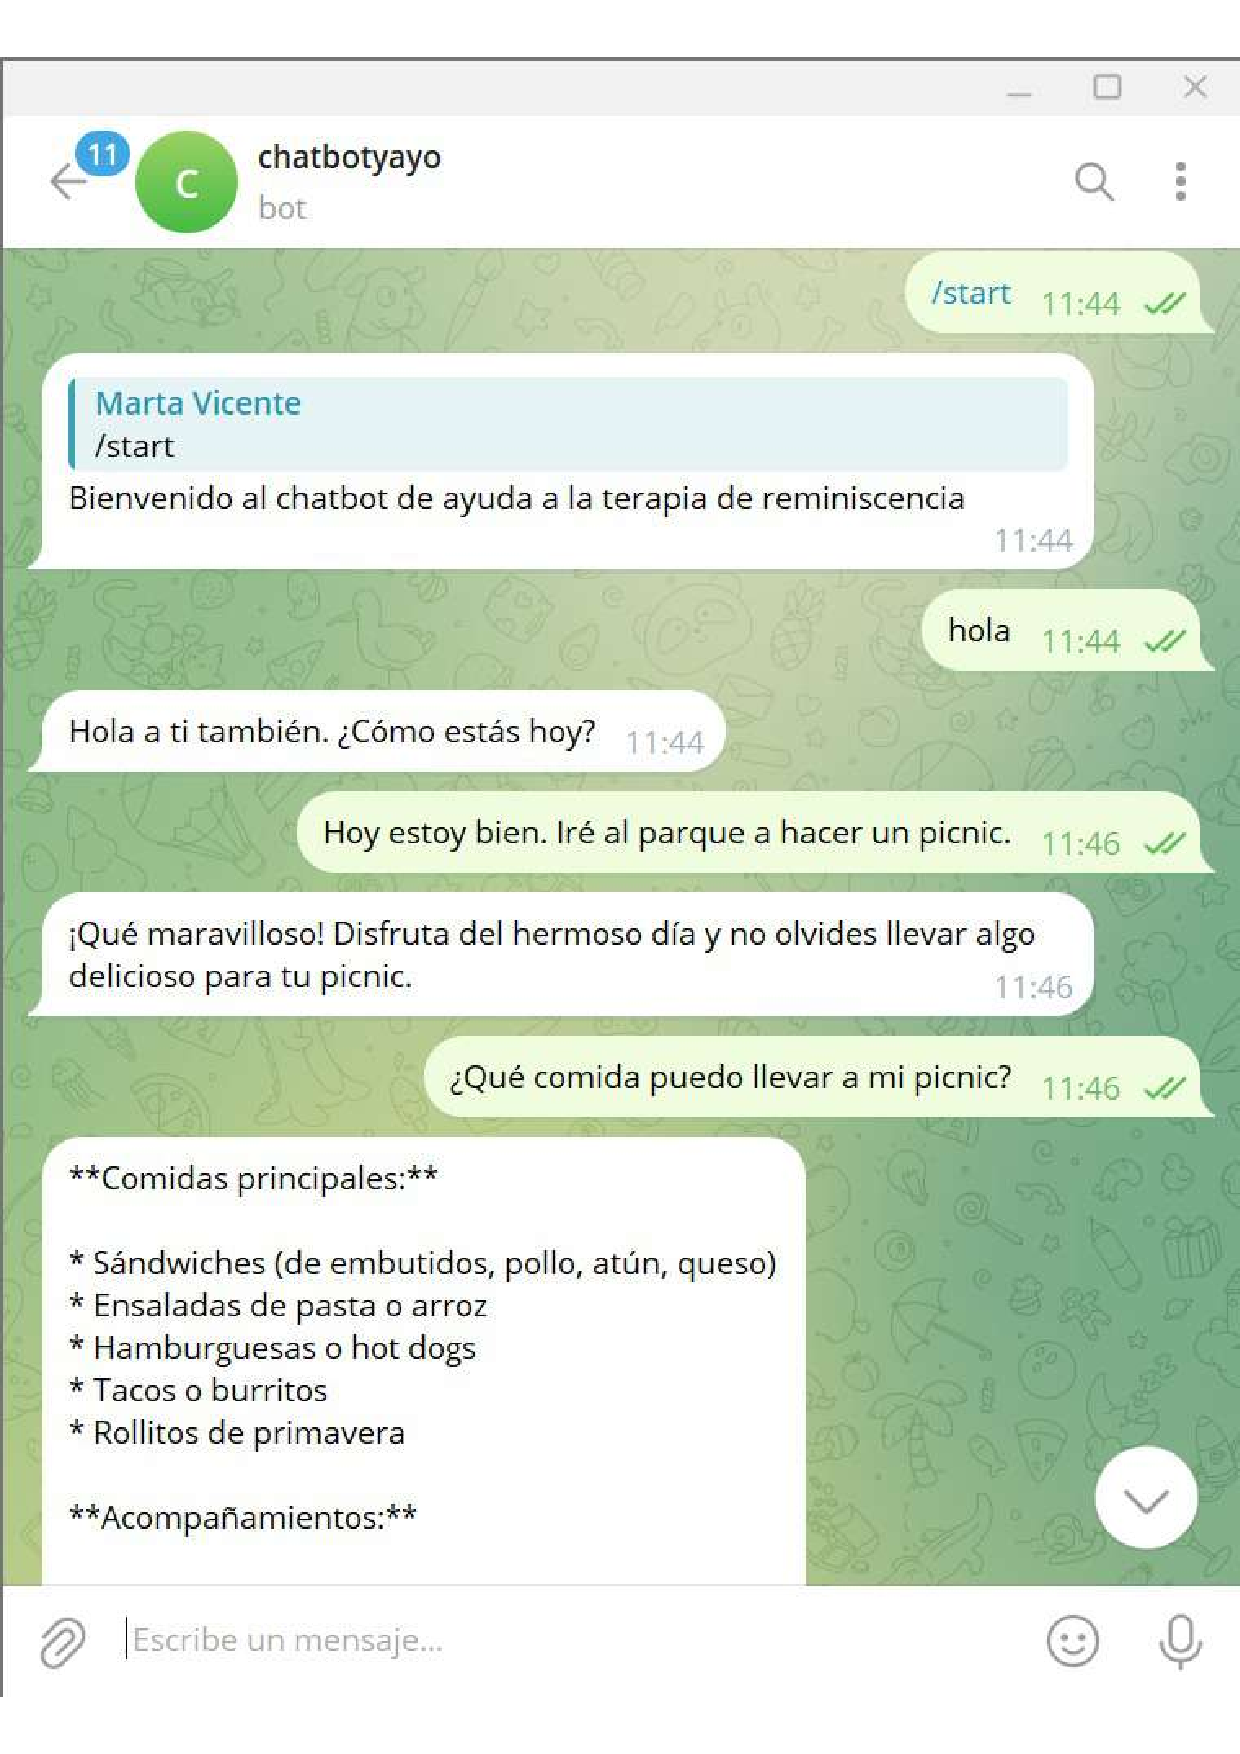
\includegraphics[width=0.5\textwidth]{Imagenes/telegram1}

%PRIMERA VERSIÓN EN BARD
%PRIMERA VERSIÓN EN GEMMA
%PRIMERA VERSIÓN GEMINI - GOOGLE COLLABORATE
%REFACTORIZACIÓN PARA HACER VERSIÓN LOCAL
%TELEGRAM
%GENERAR LAS ETAPAS 
%IMAGENES
%WHISPER
%GRÁFOS
%GENERACIÓN DE HISTORIAS DE VIDA
Para configurarlo, en primer lugar hay que ejecutar el programa mibot.py estando en telegram en la conversaa conversación de telegram el comando /start para comenzar la conversación y ya. 

Sin embago, y pese a las grandes funcionalidades de todas estas alternativas nos hemos decantado por hacer una interfaz con telegram desarrollando nuestro propio chatbot usando rasa. 

Para desarrollar el chatbot de telegram me he decantado por usar la interfaz de telegram para la cuál se necesita la API de Rasa. Las principales ventajas que ofrece esta herramienta es la facilidad del manejo de la interfaz pues telegram es una herramienta muy conocida con la que los terapeutas pueden estar más familiarizados. Además, esto nos permite también usar la versión del chatbotyayo para móvil. 

Para crear está interfaz hay que: 
1. Instalar rasa
2. Instalar telegram 
2. Obtener una api de rasa
4. crear un nuevo chatbot desde telegram con @botFather
5. Enviar a tu chatbot el comando /start

Una vez seguidos todos estos pasos ya puedes comenzar a interactuar con la API de rasa. 


\section{Respuestas de Gemini}

El modelo más apropiado para el procesamiento de texto es $gemini-pro$. La estructura de las respuestas de este modelo es la siguiente. 

\begin{lstlisting}[style=SpyderStyle, caption={Estructura de una respuesta de Gemini}, captionpos=b, label={lst:python},breaklines = true]
{
	"candidates": [
	{
		"content": {
			"parts": [
			{
				"text": string
			}
			]
		},
		"finishReason": enum (FinishReason),
		"safetyRatings": [
		{
			"category": enum (HarmCategory),
			"probability": enum (HarmProbability),
			"blocked": boolean
		}
		],
		"citationMetadata": {
			"citations": [
			{
				"startIndex": integer,
				"endIndex": integer,
				"uri": string,
				"title": string,
				"license": string,
				"publicationDate": {
					"year": integer,
					"month": integer,
					"day": integer
				}
			}
			]
		}
	}
	],
	"usageMetadata": {
		"promptTokenCount": integer,
		"candidatesTokenCount": integer,
		"totalTokenCount": integer
	}
}
\end{lstlisting}

\begin{itemize}
\item \textbf{text}	El texto generado.
\item \textbf{finishReason}	El motivo por el que el modelo dejó de generar tokens. Si está vacío, el modelo no dejó de generar los tokens. El motivo puede ser cualquiera de los siguientes:
\begin{enumerate}
	\item $FINISH\_REASON\_UNSPECIFIED$: no se especifica el motivo de finalización.
	\item $FINISH\_REASON\_STOP$: punto de detención natural del modelo o secuencia de detención proporcionada.
	\item $FINISH\_REASON\_MAX\_TOKENS$: se alcanzó la cantidad máxima de tokens especificada en la solicitud.
	\item $FINISH\_REASON\_SAFETY$: la generación del token se detuvo porque la respuesta se marcó por motivos de seguridad. Ten en cuenta que Candidate.content está vacío si los filtros de contenido bloquean el resultado.
	\item $FINISH\_REASON\_RECITATION$: la generación del token se detuvo porque la respuesta se marcó para citas no autorizadas.
	\item $FINISH\_REASON\_OTHER$: todos los demás motivos que detuvieron el token
\end{enumerate}

\item \textbf{category}	La categoría de seguridad para la que se configura un umbral. Los valores aceptables son los siguientes:
Haz clic para expandir las categorías de seguridad
\begin{enumerate}
	\item $HARM\_CATEGORY\_SEXUALLY\_EXPLICIT$
	\item $HARM\_CATEGORY\_HATE\_SPEECH$
	\item $HARM\_CATEGORY\_HARASSMENT$
	\item $HARM\_CATEGORY\_DANGEROUS\_CONTENT$
\end{enumerate}
\item \textbf{probability}	Los niveles de probabilidad de daños en el contenido.
\begin{enumerate}
	\item $HARM\_PROBABILITY\_UNSPECIFIED$
	\item $NEGLIGIBLE$
	\item $LOW$
	\item $MEDIUM$
	\item $HIGH$
\end{enumerate}
\item \textbf{blocked}	Una marca boolean asociada con un atributo de seguridad que indica si la entrada o salida del modelo se bloqueó. Si blocked es true, el campo errors en la respuesta contiene uno o más códigos de error. Si blocked es false, la respuesta no incluye el campo errors.
\item \textbf{startIndex}	Un número entero que especifica dónde comienza una cita en el contenido.
\item \textbf{endIndex}	Un número entero que especifica dónde termina una cita en content.
\item \textbf{url}	Es la URL de una fuente de cita. Los ejemplos de una fuente de URL pueden ser un sitio web de noticias o un repositorio de GitHub.
\item \textbf{title}	Es el título de una fuente de cita. Los ejemplos de títulos de origen pueden ser los de un artículo de noticias o un libro.
\item \textbf{license}	Es la licencia asociada con una cita.
\item \textbf{publicationDate}	La fecha en que se publicó una cita. Sus formatos válidos son YYYY, YYYY-MM y YYYY-MM-DD.
\item \textbf{promptTokenCount}	Cantidad de tokens en la solicitud.
\item \textbf{candidatesTokenCount}	Cantidad de tokens en las respuestas.
\item \textbf{totalTokenCount}	Cantidad de tokens en la solicitud y las respuestas.
\end{itemize}
\chapter{ChatBot final}
\label{cap:ChatBot final}
\section{Arquitectura}
\section{Herramientas y puesta en marcha}
\subsection{VPN}
\section{Implementación de las funcionalidades}
\subsection{Extracción de la información}
\subsection{Generación de preguntas}
\subsection{Interfaz e interacción con el usuario}
\subsection{Almacenamiento de la información}

%IDEA AÑADIR SECCIÓN EVALUACIÓN
\chapter{Conclusiones y Trabajo Futuro}
\label{cap:conclusiones}

Conclusiones del trabajo y líneas de trabajo futuro.

Antes de la entrega de actas de cada convocatoria, en el plazo que se indica en el calendario de los trabajos de fin de grado, el estudiante entregará en el Campus Virtual la versión final de la memoria en PDF.



\begin{otherlanguage}{english}
	\chapter*{Conclusions and Future Work}
\label{cap:conclusions}
\addcontentsline{toc}{chapter}{Conclusions and Future Work}
This chapter describes the conclusions reached after months of work on a project to build a conversational tool to help reminiscence therapy. Despite the exponential development that AI is undergoing in the field of language processing, the provisional nature of the models and the constant changes in the legislation of the territories have led to various problems and consequently to a much broader study of the current situation and the different alternatives.

In this chapter, we do not only intend to talk about the conclusions about the developed tool, but also about all the conclusions associated with the previous theoretical study.

On the other hand, possible future works that can be considered as a result of the research will be described.

\section{Actual state of PLN}
In recent years, the progress in language processing has been notable, with numerous advantages, but also with risks associated with software development.

On the one hand, artificial intelligence models evolve rapidly, generating frequent updates labeled as "latest stable version." This designation refers to the most recent version of the model that has been tested and validated for widespread use, offering quality and reliability \cite{generative-ai-terms}.

On the other hand, AIs face the problem of regulation. The President of the European Commission, Ursula von der Leyen, has underlined that AI is transforming our lives and has emphasized the importance of a sensible and widespread approach to benefit the economy and society \cite{ComisionEuropea-ComunicadoPrensa-LeyIA}. The recently approved EU AI Law, considered the first global framework on this matter, seeks to promote responsible innovation by regulating identified risks and guaranteeing the safety and fundamental rights of people and companies.

This approach is based on assessing the risk of AI systems: those with low risk, such as recommendation systems, will have freedom and no obligation, while those with high risk, such as critical infrastructures, health systems and police applications, will have to meet strict mitigation, data quality, and human oversight requirements. In addition, AI systems that pose a clear threat to fundamental rights, such as the manipulation of human behavior, will be banned. Specific rules will be introduced to ensure transparency in general-purpose AI models, along with fines for companies that do not comply with regulations.


In December 2023, a draft on the regulation of AI by the Council of the European Union and the European Parliament was prepared. Finally, on February 2, 2024, first law on artificial intelligence was passed, the AI Act. After a meeting in Brussels, the ambassadors of the 27 Member States gave their political approval to this regulation, following the presentation in January of the final version of the text and the creation of the European Artificial Intelligence Office. Although some countries showed opposition until the last moment, the path continued its course and it is expected that between 2024 and 2030 all countries will adopt the law \cite{ElDerecho-LeyIA}.

Constant changes in models and modifications in national legislation pose a challenge for software developers. During the development of this project, we faced various situations derived from these events. On the one hand, we had to look for an alternative to the Bard API, which was transformed into Gemini between December 2023 and February 2024, and on the other hand, face the limitations imposed by the different laws, which were solved through the VPN use.

In fact, the situation is changing so quickly that in the final stretch of the project we have observed several changes in the terms and conditions of use of the Gemini API worldwide. In fact, the next update of the terms of use will be May 22, 2024.

In conclusion, in the field of language development and information extraction from images, AI is experiencing numerous advances in recent years. However, it is essential to keep in mind that the use of the different models is subject to changes both in the versions and their characteristics, as well as in the laws and terms and conditions of use.
\section{Project development}
To begin developing this work, the first step is to be clear about its objectives and requirements. Analyze the problem in relation to other existing work to develop a useful tool.

After establishing the objectives and requirements of our project in a general way, the next step is to present them in a more technical and detailed way. To do this, we designed an architecture based on the various tasks that the system had to carry out. However, before implementing the system, some issues related to certain components of the architecture arose.

Mainly, we had to resolve the appropriate selection of the language model to use, given the wide variety of models available. Additionally, we needed to ensure access to an adequate data set relevant to the biodata transformation objectives, allowing the model to be adjusted effectively.
For the development of the main core of the system, the module responsible for processing incoming information, numerous prototypes were developed, the most important of which are explained in the chapter \ref{cap:Desarrollo de prototipos}.

The main challenge of this project has undoubtedly been facing all those version changes, updates and changes in legislation that altered the operation of the model. Much of the time dedicated to this work has been focused on research into different language processing tools.

Once the final model, Gemini, has been selected and everything necessary for its implementation has been carried out, the central stage of development begins following the explained incremental design plan \ref{sec:objectivos}.

Finally, the model was applied to obtain results and analyze its behavior.


\section{Final result}
As a result of the development of this project, a conversational tool has been created to support reminiscence therapy. The main function of this bot is to search and store relevant information to generate life stories using other tools. The intuitive and easy-to-use user interface makes this tool accessible not only to therapists, but also to family members and patients who are familiar with mobile devices and computers.

Although initially designed as a therapeutic tool to gather information about the patient's life, this tool has multiple uses. For example, portable versions, such as the mobile or tablet app, allow for use as entertainment during long trips that can be challenging for patients. In addition, the ease of use also allows patients to use it in moments of solitude, having interesting conversations about their life that stimulate the mind and provide them with virtual companionship.

\section{Future work}

As a final point of this work, those possible open lines of development and research are exposed, which have emerged after the analysis of the project, and which could be studied with the aim of improving the project.

Firstly, although this work generates a small life story as the final result of the conversation, it would be interesting to connect this work with the project explained in the section \ref{sec:trabajocristina} ``Generation of life stories using Deep Learning techniques ''. To do this, it would be interesting to transform all the information obtained through the conversation with this chatbot into an input set with the appropriate format for the application developed in that work. In this way, life stories that are more faithful to the person's real life would be generated, and the full cycle of work prior to reminiscence therapy would be completed.

On the other hand, another modification that could be interesting would be the adaptation of the model to multiples lenguages, in order to expand the public target. The Gemini API is available in different languages, but the handling of all predefined questions would have to be translated for user interaction.

The development of the Gemini API, and the access of new versions will bring new possibilities. Among them, the integration of videos to send to the chatbot stands out, which are analyzed with the aim of obtaining more bibliographic information. It may also be interesting to consider the alternative of voice recognition so that in addition to the Telegram interface, a voice interface could be developed where the patient could speak and listen as if it were a phone call.

\end{otherlanguage}

% Bibliografía
%
% Si el TFM se escribe en inglés, editar TeXiS/TeXiS_bib para cambiar el
% estilo de las referencias
%---------------------------------------------------------------------
%
%                      configBibliografia.tex
%
%---------------------------------------------------------------------
%
% bibliografia.tex
% Copyright 2009 Marco Antonio Gomez-Martin, Pedro Pablo Gomez-Martin
%
% This file belongs to the TeXiS manual, a LaTeX template for writting
% Thesis and other documents. The complete last TeXiS package can
% be obtained from http://gaia.fdi.ucm.es/projects/texis/
%
% Although the TeXiS template itself is distributed under the 
% conditions of the LaTeX Project Public License
% (http://www.latex-project.org/lppl.txt), the manual content
% uses the CC-BY-SA license that stays that you are free:
%
%    - to share & to copy, distribute and transmit the work
%    - to remix and to adapt the work
%
% under the following conditions:
%
%    - Attribution: you must attribute the work in the manner
%      specified by the author or licensor (but not in any way that
%      suggests that they endorse you or your use of the work).
%    - Share Alike: if you alter, transform, or build upon this
%      work, you may distribute the resulting work only under the
%      same, similar or a compatible license.
%
% The complete license is available in
% http://creativecommons.org/licenses/by-sa/3.0/legalcode
%
%---------------------------------------------------------------------
%
% Fichero  que  configura  los  parámetros  de  la  generación  de  la
% bibliografía.  Existen dos  parámetros configurables:  los ficheros
% .bib que se utilizan y la frase célebre que aparece justo antes de la
% primera referencia.
%
%---------------------------------------------------------------------


%%%%%%%%%%%%%%%%%%%%%%%%%%%%%%%%%%%%%%%%%%%%%%%%%%%%%%%%%%%%%%%%%%%%%%
% Definición de los ficheros .bib utilizados:
% \setBibFiles{<lista ficheros sin extension, separados por comas>}
% Nota:
% Es IMPORTANTE que los ficheros estén en la misma línea que
% el comando \setBibFiles. Si se desea utilizar varias líneas,
% terminarlas con una apertura de comentario.
%%%%%%%%%%%%%%%%%%%%%%%%%%%%%%%%%%%%%%%%%%%%%%%%%%%%%%%%%%%%%%%%%%%%%%
\setBibFiles{%
	biblio%
	}

%%%%%%%%%%%%%%%%%%%%%%%%%%%%%%%%%%%%%%%%%%%%%%%%%%%%%%%%%%%%%%%%%%%%%%
% Definición de la frase célebre para el capítulo de la
% bibliografía. Dentro normalmente se querrá hacer uso del entorno
% \begin{FraseCelebre}, que contendrá a su vez otros dos entornos,
	% un \begin{Frase} y un \begin{Fuente}.
			%
			% Nota:
			% Si no se quiere cita, se puede eliminar su definición (en la
			% macro setCitaBibliografia{} ).
			%%%%%%%%%%%%%%%%%%%%%%%%%%%%%%%%%%%%%%%%%%%%%%%%%%%%%%%%%%%%%%%%%%%%%%
			%\setCitaBibliografia{
			%	\begin{FraseCelebre}
			%		\begin{Frase}
			%			Y así, del mucho leer y del poco dormir, se le secó el celebro de
			%			manera que vino a perder el juicio.\\ 
			%		\end{Frase}
			%		\begin{Fuente}
			%			Miguel de Cervantes Saavedra
			%		\end{Fuente}
			%	\end{FraseCelebre}
			%}
			
			

\makeBib

% Apéndices
\appendix
\chapter{Título del Apéndice A}
\label{Appendix:Key1}

Los apéndices son secciones al final del documento en las que se agrega texto con el objetivo de ampliar los contenidos del documento principal.
%\chapter{Título del Apéndice B}
\label{Appendix:Key2}

Se pueden añadir los apéndices que se consideren oportunos.
%\include{Apendices/appendixC}
%\include{...}
%\include{...}
%\include{...}
\backmatter



%
% Índice de palabras
%

% Sólo  la   generamos  si  está   declarada  \generaindice.  Consulta
% TeXiS.sty para más información.

% En realidad, el soporte para la generación de índices de palabras
% en TeXiS no está documentada en el manual, porque no ha sido usada
% "en producción". Por tanto, el fichero que genera el índice
% *no* se incluye aquí (está comentado). Consulta la documentación
% en TeXiS_pream.tex para más información.
\ifx\generaindice\undefined
\else
%%---------------------------------------------------------------------
%
%                        TeXiS_indice.tex
%
%---------------------------------------------------------------------
%
% TeXiS_indice.tex
% Copyright 2009 Marco Antonio Gomez-Martin, Pedro Pablo Gomez-Martin
%
% This file belongs to TeXiS, a LaTeX template for writting
% Thesis and other documents. The complete last TeXiS package can
% be obtained from http://gaia.fdi.ucm.es/projects/texis/
%
% This work may be distributed and/or modified under the
% conditions of the LaTeX Project Public License, either version 1.3
% of this license or (at your option) any later version.
% The latest version of this license is in
%   http://www.latex-project.org/lppl.txt
% and version 1.3 or later is part of all distributions of LaTeX
% version 2005/12/01 or later.
%
% This work has the LPPL maintenance status `maintained'.
% 
% The Current Maintainers of this work are Marco Antonio Gomez-Martin
% and Pedro Pablo Gomez-Martin
%
%---------------------------------------------------------------------
%
% Contiene  los  comandos  para  generar  el índice  de  palabras  del
% documento.
%
%---------------------------------------------------------------------
%
% NOTA IMPORTANTE: el  soporte en TeXiS para el  índice de palabras es
% embrionario, y  de hecho  ni siquiera se  describe en el  manual. Se
% proporciona  una infraestructura  básica (sin  terminar)  para ello,
% pero  no ha  sido usada  "en producción".  De hecho,  a pesar  de la
% existencia de  este fichero, *no* se incluye  en Tesis.tex. Consulta
% la documentación en TeXiS_pream.tex para más información.
%
%---------------------------------------------------------------------


% Si se  va a generar  la tabla de  contenidos (el índice  habitual) y
% también vamos a  generar el índice de palabras  (ambas decisiones se
% toman en  función de  la definición  o no de  un par  de constantes,
% puedes consultar modo.tex para más información), entonces metemos en
% la tabla de contenidos una  entrada para marcar la página donde está
% el índice de palabras.

\ifx\generatoc\undefined
\else
   \addcontentsline{toc}{chapter}{\indexname}
\fi


% Generamos el índice
\printindex

% Variable local para emacs, para  que encuentre el fichero maestro de
% compilación y funcionen mejor algunas teclas rápidas de AucTeX

%%%
%%% Local Variables:
%%% mode: latex
%%% TeX-master: "./tesis.tex"
%%% End:

\fi

%
% Lista de acrónimos
%

% Sólo  lo  generamos  si  está declarada  \generaacronimos.  Consulta
% TeXiS.sty para más información.


\ifx\generaacronimos\undefined
\else
%---------------------------------------------------------------------
%
%                        TeXiS_acron.tex
%
%---------------------------------------------------------------------
%
% TeXiS_acron.tex
% Copyright 2009 Marco Antonio Gomez-Martin, Pedro Pablo Gomez-Martin
%
% This file belongs to TeXiS, a LaTeX template for writting
% Thesis and other documents. The complete last TeXiS package can
% be obtained from http://gaia.fdi.ucm.es/projects/texis/
%
% This work may be distributed and/or modified under the
% conditions of the LaTeX Project Public License, either version 1.3
% of this license or (at your option) any later version.
% The latest version of this license is in
%   http://www.latex-project.org/lppl.txt
% and version 1.3 or later is part of all distributions of LaTeX
% version 2005/12/01 or later.
%
% This work has the LPPL maintenance status `maintained'.
% 
% The Current Maintainers of this work are Marco Antonio Gomez-Martin
% and Pedro Pablo Gomez-Martin
%
%---------------------------------------------------------------------
%
% Contiene  los  comandos  para  generar  el listado de acrónimos
% documento.
%
%---------------------------------------------------------------------
%
% NOTA IMPORTANTE:  para que la  generación de acrónimos  funcione, al
% menos  debe  existir  un  acrónimo   en  el  documento.  Si  no,  la
% compilación  del   fichero  LaTeX  falla  con   un  error  "extraño"
% (indicando  que  quizá  falte  un \item).   Consulta  el  comentario
% referente al paquete glosstex en TeXiS_pream.tex.
%
%---------------------------------------------------------------------


% Redefinimos a español  el título de la lista  de acrónimos (Babel no
% lo hace por nosotros esta vez)

\def\listacronymname{Lista de acrónimos}

% Para el glosario:
% \def\glosarryname{Glosario}

% Si se  va a generar  la tabla de  contenidos (el índice  habitual) y
% también vamos a  generar la lista de acrónimos  (ambas decisiones se
% toman en  función de  la definición  o no de  un par  de constantes,
% puedes consultar config.tex  para más información), entonces metemos
% en la  tabla de contenidos una  entrada para marcar  la página donde
% está el índice de palabras.

\ifx\generatoc\undefined
\else
   \addcontentsline{toc}{chapter}{\listacronymname}
\fi


% Generamos la lista de acrónimos (en realidad el índice asociado a la
% lista "acr" de GlossTeX)

\printglosstex(acr)

% Variable local para emacs, para  que encuentre el fichero maestro de
% compilación y funcionen mejor algunas teclas rápidas de AucTeX

%%%
%%% Local Variables:
%%% mode: latex
%%% TeX-master: "../Tesis.tex"
%%% End:

\fi

%
% Final
%
%---------------------------------------------------------------------
%
%                      fin.tex
%
%---------------------------------------------------------------------
%
% fin.tex
% Copyright 2009 Marco Antonio Gomez-Martin, Pedro Pablo Gomez-Martin
%
% This file belongs to the TeXiS manual, a LaTeX template for writting
% Thesis and other documents. The complete last TeXiS package can
% be obtained from http://gaia.fdi.ucm.es/projects/texis/
%
% Although the TeXiS template itself is distributed under the 
% conditions of the LaTeX Project Public License
% (http://www.latex-project.org/lppl.txt), the manual content
% uses the CC-BY-SA license that stays that you are free:
%
%    - to share & to copy, distribute and transmit the work
%    - to remix and to adapt the work
%
% under the following conditions:
%
%    - Attribution: you must attribute the work in the manner
%      specified by the author or licensor (but not in any way that
%      suggests that they endorse you or your use of the work).
%    - Share Alike: if you alter, transform, or build upon this
%      work, you may distribute the resulting work only under the
%      same, similar or a compatible license.
%
% The complete license is available in
% http://creativecommons.org/licenses/by-sa/3.0/legalcode
%
%---------------------------------------------------------------------
%
% Contiene la última página
%
%---------------------------------------------------------------------


% Ponemos el marcador en el PDF
\ifpdf
   \pdfbookmark{Fin}{fin}
\fi

\thispagestyle{empty}\mbox{}

Este texto se puede encontrar en el fichero Cascaras/fin.tex. Si deseas eliminarlo, basta con comentar la línea correspondiente al final del fichero TFGTeXiS.tex.

\vspace*{4cm}

\small

\hfill \emph{--¿Qué te parece desto, Sancho? -- Dijo Don Quijote --}

\hfill \emph{Bien podrán los encantadores quitarme la ventura,}

\hfill \emph{pero el esfuerzo y el ánimo, será imposible.}

\hfill 

\hfill \emph{Segunda parte del Ingenioso Caballero} 

\hfill \emph{Don Quijote de la Mancha}

\hfill \emph{Miguel de Cervantes}

\vfill%space*{4cm}

\hfill \emph{--Buena está -- dijo Sancho --; fírmela vuestra merced.}

\hfill \emph{--No es menester firmarla -- dijo Don Quijote--,}

\hfill \emph{sino solamente poner mi rúbrica.}

\hfill 

\hfill \emph{Primera parte del Ingenioso Caballero} 

\hfill \emph{Don Quijote de la Mancha}

\hfill \emph{Miguel de Cervantes}


\newpage
\thispagestyle{empty}\mbox{}

\newpage

% Variable local para emacs, para  que encuentre el fichero maestro de
% compilación y funcionen mejor algunas teclas rápidas de AucTeX

%%%
%%% Local Variables:
%%% mode: latex
%%% TeX-master: "../Tesis.tex"
%%% End:

%\end{otherlanguage}
\end{document}
